An electron bubble is a stable configuration that a free electron acquires in liquid helium. \cite{Classen} The electron is repelled by a helium atom because if it tries to pass through the atom, it has to go into a n=2 state. This makes the energy of the electron about 1 eV higher than the energy in the vacuum. But, it turns out that, the electron can lower its energy by creating a bubble in the liquid that is free of helium atoms. The electron losses its energy either by scattering helium atoms, by ionizing helium atoms, or by exciting the atoms. The formation of the electron bubble is demonstrated in Fig. \ref{bubbleFormation}.
\begin{figure}[H]
\centering 
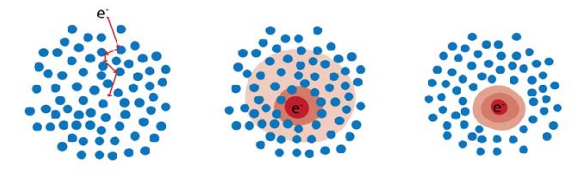
\includegraphics[width=100mm, height=30mm]{Introduction/bubbleFormation.png}
\caption{Process for formation of electron bubbles. \cite{Yang2018thesis}}
\label{bubbleFormation}
\end{figure}

The energy of this bubble can be be approximated as follows:
\begin{equation}\label{energyEqbub}
E=\frac{h^2}{8mR^2}+4\pi R^2\alpha + \frac{4}{3}\pi R^3 P
\end{equation}
where $\alpha$ is surface tension, $R$ is the radius of the bubble, $h$ is Plank's constant, $m$ is the mass of an electron, and $P$ is the applied pressure. Equation \ref{energyEqbub} can be understood as the sum of zero-point energy of the electron (the energy of electron due to being confined in a potential well that is the bubble), the surface energy of the bubble, and the volume energy of the bubble: the work done while creating the bubble over pressure $P$.  

If we assume that $P=0$, differentiating Eq. \ref{energyEqbub} and setting it to zero, the energy has a minimum at
\begin{equation}\label{minEnergy}
R_{min} = \left(\frac{h^2}{32\pi m \alpha}\right)^{1/4}
\end{equation} 
From Eq. the \ref{minEnergy}, value of $R_{min}$ is $19 \AA$ at $0K$. This gives a good intuition of how big electron bubbles are. These bubbles are subjects of ongoing research and have led to many surprising results. 

In one such experiment, electron bubbles were subjected to an applied electric field. \cite{Wei2016} The goal was to determine the mobility of electron bubbles in superfluid helium where the mobility is restricted mainly by thermal excitation: phonons and rotons (explained in detail in Chapter 2). In this experiment, electron bubbles were introduced at the top of a cell containing liquid and the time it takes for them to reach the bottom positive plate was recorded. They were expected to reach the bottom plate about the same time since electron bubbles all have the same mobility. Thus it was expected that there would be a sharp decline in voltage when these electron bubbles reached the bottom plate. This voltage change was indeed observed, but as the Fig. \ref{exo_ions} shows there were other bubbles which traveled faster than ordinary electron bubbles and arrive quicker.  
\begin{figure}[H]
\centering 
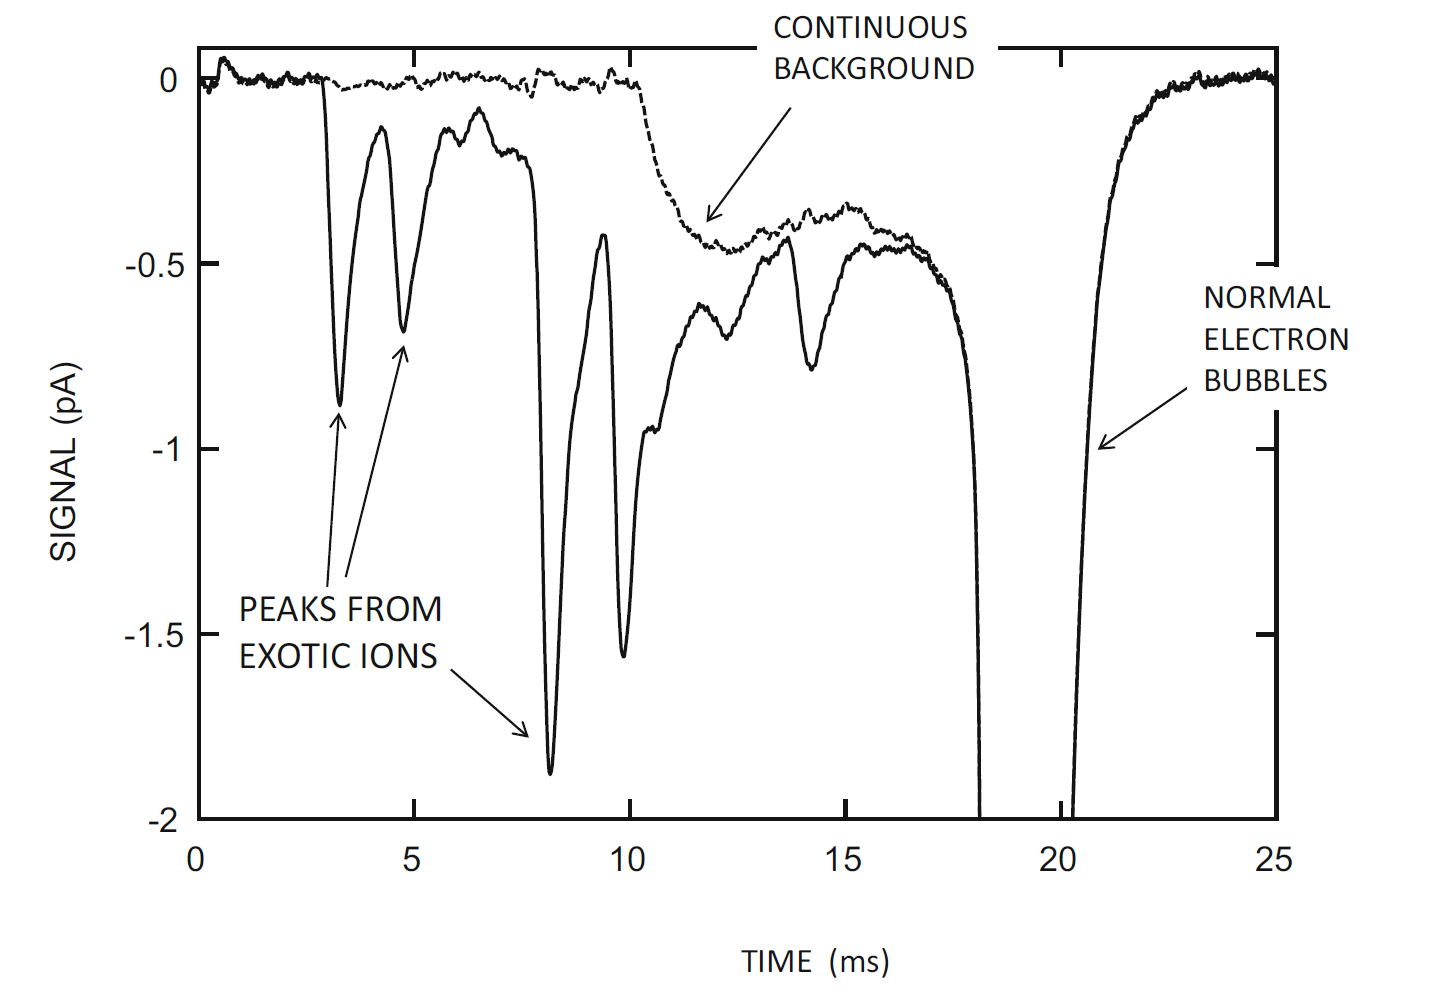
\includegraphics[width=110mm, height=80mm]{Introduction/exo_ions.png}
\caption{Solid curve showing the current arriving at the collector as a function of time. \cite{Wei2016}}
\label{exo_ions}
\end{figure}

The first ion to reach the detector was termed fast ion and was first observed by Doake and Gribbon. Shortly after the discovery of the fast ion, Ihas and Sanders discovered several other ions having mobility between the fast ion and the electron bubble. To this date, at least 18 such ions have been observed. A continuous background is also observed. This background is quite surprising since it implies that there are ions that have a continuous distribution of size. These bubbles are called the exotic ions and appear to be smaller than ordinary electron bubbles.

There is no general explanation for the existence of exotic ions. One might consider that they are impurities in liquid helium; however, that would imply that there are 18 different impurities in liquid helium. This is not probable since the number density of impurities in liquid helium is expected to be very small. Another possible explanation is that the exotic ions are negatively charged helium atoms. While it is true that ions of both helium atoms and helium dimers have been observed, they cannot explain the continuous background. Moreover, their lifetime is quite short. Therefore, it is unlikely that they pass through the mobility cell in the experiments-- where the time has been as large as $100 ms$.

Considering the bubble as a Quantum Mechanical system might provide a solution. The proposed fission model suggests that the exotic ions are bubbles that contain a fraction of the total wave function of an electron. If a fraction of the wave function, $\psi$, is in a bubble, then the bubble would be smaller in size than an electron bubble. The integral of $|\psi^2|$ over the bubble could have a continuous range of values and that could potentially explain the continuous background. A detailed mathematical analysis can be found in \cite{Wei2016}.

A further investigation is needed in order to understand the structure and origin of exotic ions. However, much simpler experiments need to be performed on electron bubbles before designing experiments for exotic ions. This is because electron bubbles are relatively well understood and have been studied for a long time. This thesis reports one such experiment.

Our experiment involved studying the effects of sound waves on electrons bubbles. This was done by introducing a negative pressure to an electron bubble at the focus of a piezoelectric transducer. The critical pressure at which an electron bubble bursts was studied against temperature, static pressure and frequency of sound.